\section{Search for CSP}

Arc consistency can effectively limit the valid domains of a CSP, but in general to actually find a complete consistent assignment we may have to return to running a search-like algorithm. (However we will see a different approach in the next section).
Here is the search model for solving CSPs:

\begin{center}
\begin{tabularx}{\linewidth}{llX}
  \toprule
  Name (AIMA) & Type & Description \\
  \midrule
\\
 State space & $\mcS$ & \censor{All possible \textbf{consistent} CSP assignments (possible partial).} \\\\
 Action model&  $\msc{Actions}$ & \censor{All consistent assignments to any unassigned variable.} \\\\
 Transition model&  $\msc{Result} $ &  \censor{A new consistent assignment after assigning an unassigned variable.}  \\\\
 Initial state &  $s_0 \in \mcS$ & \censor{The partial assignment with all variables blank, i.e. $\epsilon$ .}  \\\\
 Goal test& $\msc{Goal}: \mcS \rightarrow \{0, 1\}$ & \censor{Any complete consistent assignment.} \\\\
 \bottomrule
\end{tabularx}
\end{center}

\noindent As with game playing we will  use the recursive, tree-search version of 
DFS for this problem.

\begin{exercise}
  Why not use BFS or UCS for this problem? Why not graph search? What are the search properties of this model?
\end{exercise}

\censor{}

\air

Below is the recursive DFS algorithm. It adds a couple of elements to standard DFS. First it checks if an action is valid by ensuring that the
new CSP state is a consistent assignment. Second at  each  
step it runs a round of \textsc{Inference},  
which may consists of running arc consistency as above to limit the future domains. AIMA 
also describes various other inference steps that are specific to 
special types of factors.

\begin{algorithm}[h]
\begin{algorithmic}[1]
  \Require{$A$ is consistent assignment}
  \Ensure{true if complete, consistent assignment is found}
  \Procedure{Backtrack}{$A$}
  \If{$A$ is complete}
  \Return{$A$}
  \EndIf{}
  \State{$X_i \gets$ variable with $A_i = \epsilon$}
  \For{$x \in \mcD_i$ in pre-selected order}
  \If{$x$ is consistent with assignment }
  \State{$A_i \gets x$}
  \State{check  $\gets \msc{ForwardCheck}(A)$}
  \If{$\lnot$ check} \Return{false}
  \EndIf{}
  % \State{$\msc{ForwardCheck}(A)$}
  \State{result $\gets \msc{Backtrack}(A)$}
  \If{result } \Return{true}

  \EndIf{}
  \State{undo $\msc{ForwardCheck}(A)$}
  \State{$A_i \gets \epsilon$}

  \EndIf{}
  \EndFor{}
  \State{\Return{false}}
  \EndProcedure{}
\end{algorithmic}
\end{algorithm}

\subsection{Ordering Heuristics}
  
Finally of special concern for CSPs is selecting the order in which DFS 
proceeds. CSPs often have a very large branching factor $O(n^{D^*})$ where 
$D^*$ is the size of the largest domain $D^* = \max_{i} |\mcD_i|$. Therefore 
there has been research into selecting the order for expanding future 
assignments of a given state. In particular in the homework you will explore a few variants of this search algorithm.

\begin{exercise}
  For the homework you will implement a Sudoku solver. As practice spend, spend time filling out the puzzle below.
\end{exercise}

\begin{center}
  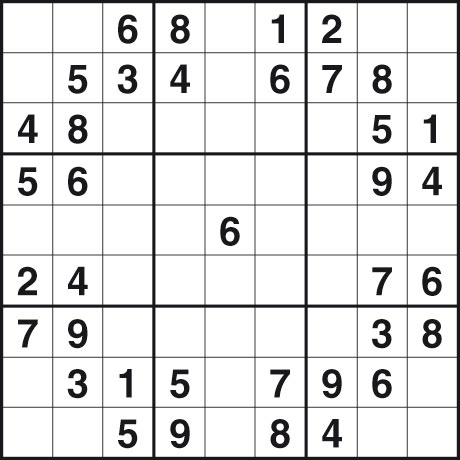
\includegraphics[width=5cm]{../pics/sudoku}
\end{center}

\begin{exercise}
  Given the puzzle, what order should we handle unassigned variables? (line 3)
\end{exercise}

\censor{ Min-Remaining Values   Degree/ number of Factors heuristic}

\begin{exercise}
  Given the puzzle, what order should we assign values from $\mcD_i$? (line 4)
\end{exercise}
\censor{
   Least constraining value 
}
